\documentclass[11pt]{article}

\usepackage{graphicx}

% Enable references to labels in the notes
\usepackage{xr-hyper}
\externaldocument{p328_notes}
\usepackage{hyperref}

% Sans fonts
\usepackage{sfmath}
\renewcommand{\familydefault}{\sfdefault}

\newcommand{\COURSE}{PHYS328W}
\newcommand{\LABNUM}{8}
\newcommand{\TITLE}{AM Tuner and Demodulator}
\markright{\COURSE~Lab \LABNUM\ : \TITLE}

\setlength{\textwidth} {6.5 true in}
\setlength{\textheight}{9 true in}
\setlength{\hoffset}   {-0.75 true in}
\setlength{\voffset}   {-0.75 true in}
\setlength{\parindent} {12 pt}
\pagestyle{myheadings}

\begin{document}

\thispagestyle{empty}

\section*{\COURSE\ Lab \LABNUM\ : \TITLE}

\subsection*{Experiments}

\begin{figure}[h]
\centering
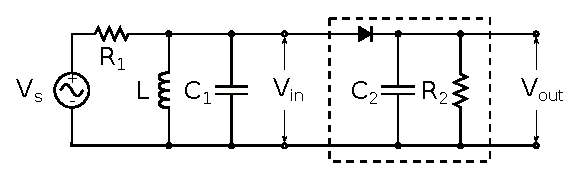
\includegraphics{demodulator.eps}
\caption{An band-pass filter driving a diode envelope
  detector in the dashed rectangle.}
\label{fig:demodulator}
\end{figure}

The circuit in Figure~\ref{fig:demodulator} (with the function
generator standing in for the antenna) is the first three stages of a
simple AM radio reciever (antenna, tuner, and demodulator). AM stands
for \textbf{amplitude modulation}. AM radio broadcasts are transmitted
at a fixed frequency, and the information is encoded as variations in
the amplitude of the carrier signal. In the United States, Radio
stations in the AM band are assigned carrier frequencies in the
535-1705~kHz range
\footnote{United States Frequency Allocation Chart,
  \url{https://www.ntia.doc.gov/files/ntia/publications/january_2016_spectrum_wall_chart.pdf},
  National Telecommunications and Information Administration
  (2016).}
at 10~kHz intervals
\footnote{NRSC-G100-A Bandwidth Options for Analog AM Broadcasters,
  \url{http://www.nrscstandards.org/sg/NRSC-G100-A.pdf},
  National Radio Systems Committee (2012)}.
In order to distinguish stations, an AM 
radio reciever must have a tuner with a bandwidth $\leq$10~kHz.  To
recover the information in the signal from an AM station, usually an
audio signal in the 100~Hz - 20 kHz range, a \textbf{demodulator} is
used to produce a signal proportional to the amplitude of the carrier
signal. A \texttt{diode envelope detector}, shown in the dashed box in
Figure~\ref{fig:demodulator} is a simple demodulator.

\begin{enumerate}
\item Construct the circuit in Figure~\ref{fig:demodulator} with the
  same $R_1$, $C_1$ and $L$ that you used in Lab 5, $C_2 = 100$~pF,
  $R_2 = 470$~k$\Omega$, and the \texttt{1N5711} small-signal Schottky
  diode. Use the function generator as your AC voltage source.

\item Drive the circuit at its resonant frequency with a sinusoidal
  signal, and display the output voltage of the tuner and the output
  voltage of the envelope detector together on the oscilloscope.
  
\item Focusing just on the output voltage of the RLC tuner (the input
  to the envelope detector), measure the resonant frequency and the
  3~dB band width of the tuner, and make note of any changes due to
  the presence of the envelope detector. 

\item Measure the amplitude of the input signal $|V_{in}|$ (the output
  of the tuner) and the size of the output signal of the envelope
  detector $|V_{out}|$.
\end{enumerate}

\subsection*{Simulations}

\subsubsection*{Comparison with Experiment}
\begin{enumerate}
\item Construct the circuit shown in Figure~\ref{fig:demodulator}
  using measured resistor, inductor, and capacitor values.

\item We need to use the specific PSpice model of the \texttt{1N5711}
  small-signal Schottky diode in this circuit. A model of this diode
  is included in the \texttt{OrCAD Capture} libraries. We need to add
  this to the schematic instead of a standard diode:
  \begin{itemize}
  \item Click the \includegraphics{OrCAD_AddPart.png} button in the
    tool bar on the right (or \texttt{Place -> Add Part ...}).

  \item The \texttt{Place Part} panel will open up on the right. In
    the \texttt{Libraries} list, select \texttt{DIODE}.

  \item Type D1N5711 into the \texttt{Part} search bar. Click on
    \texttt{D1N5711/DIODE} in the \texttt{Part List}, and hit the 
    \includegraphics{OrCAD_AddPart.png} button at the upper right of
    the \texttt{Place Part} panel (or press \texttt{Enter}) to place
    the diode in the schematic. 
  \end{itemize}

\item Set up a transient analysis over a large time scale relative to
  the 1~MHz source frequency --- say 100~$\mu$s. In order to avoid
  aliasing, set the maximum step size to 0.01~$\mu$s so that 100
  points are plotted per period.

\item As you did for the actual circuit, measure the amplitude of the
  input signal $|V_{in}|$ (the output of the tuner) and the size of
  the output signal of the envelope detector $|V_{out}|$.

\item Set up the same AC sweep analysis you used in Lab 4, and
  determine the band width of the tuner.
\end{enumerate}

\subsubsection*{Demodulation of an Amplitude-modulated Signal}
  \begin{figure}[h]
  \centering
  \scalebox{0.5}{
    \includegraphics{amplitudemod.png}
    }
  \caption{A 1~MHz sinusoidal source with 1~kHz amplitude modulation.}
  \label{fig:amplitudemod}
  \end{figure}
\begin{enumerate}
\item Make a new project, copy your existing schematic into it, and
  add a multiplier device and a second sinusoidal voltage source to
  make an amplitude-modulated source as shown in
  Figure~\ref{fig:amplitudemod}. To place a multiplier, use the
  \includegraphics{OrCAD_AddPart.png} button, select \texttt{ABM} in
  the \texttt{Libraries} panel, and select the \texttt{MULT} part in
  the \texttt{Part} panel.

\item Run a transient analysis over two periods of the 1~kHz amplitude
  modulation and measure the amplitudes $|V_{in}|$ and $|V_{out}|$.

\end{enumerate}

\subsection*{Products}

Upload to Canvas a brief \LaTeX\ report in which you ...
\begin{itemize}
\item Compare the bandwidth measurements of the RLC filter with no
  load (Lab 4) and driving the diode envelope detector. Comment on any
  discrepancies between measurements and simulations.

\item Include as a figures measured and simulated plots of $V_{in}$
  and $V_{out}$ vs. time with unmodulated and amplitude-modulated
  input signals.
\end{itemize}

\end{document}
